
\section{Kinematika robota}
\label{kap:1}

\subsection{SCARA}
\label{kap:1.1}

Scara robot je typ priemyselného robotického systému, ktorý bol vyvinutý na vykonávanie presných a opakujúcich sa úloh. Navrhol ho v roku 1979 vedec Hiroshi Makino z Yamanashi Univerzity\cite{SCARA-uvod}. Názov SCARA je akronym (Selective Compliance Assembly Robot Arm), ktorý značí, že vertikálna poddajnosť (compliance) je väčšia ako poddajnosť v horizontálnom smere. Jeho hlavnou úlohou je najčastejšie presúvanie objektov z jedného miesta na druhé. Scara roboty majú obvykle 4 stupne voľnosti a svojou konštrukciou pripomínajú ľudskú ruku. (obr. \ref{OBRAZOK 1.1}).
\begin{figure}[h]
	\centering
	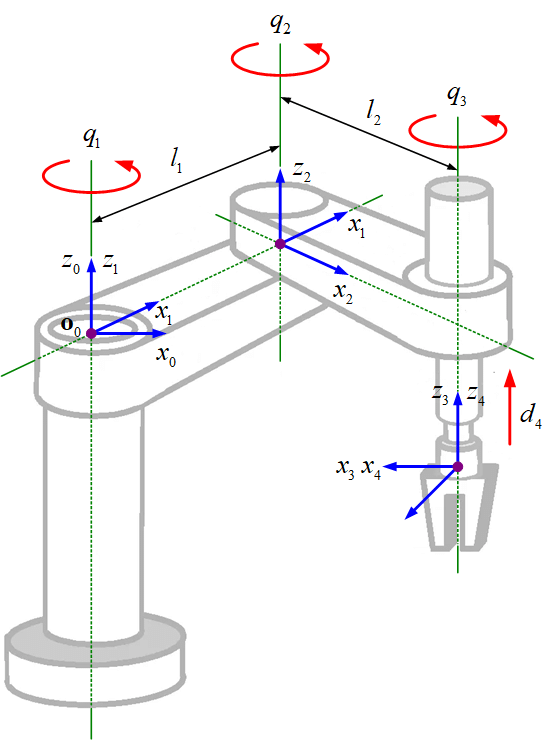
\includegraphics[width=100mm]{img/SCARA-robot-manipulator.png}
	\caption{SCARA robot - smery pohybov\cite{SCARA-struktura}}\label{OBRAZOK 1.1} 
\end{figure} 

SCARA robot disponuje tromi rotačnými kĺbmi a jedným posuvným kĺbom, ktoré mu umožňujú pohyb v priestore vo všetkých troch osiach $x$, $y$ a $z$. Tento dizajn umožňuje robotovi vykonávať presné a opakujúce sa úlohy aj keď umiestnenie rotačných kĺbov v jednej rovine obmedzuje jeho pohybovú schopnosť v porovnaní s robotmi  s robotickými ramenami so 6 stupňami voľnosti. Napriek tomu, vďaka svojej kinematickej štruktúre, SCARA roboty prinášajú niekoľko výhod, ktoré ich robia obľúbenými vo viacerých odvetviach priemyslu.

Jednou z hlavných výhod je ich schopnosť dosiahnuť vysokú presnosť a rýchlosť pri vykonávaní úloh. Navyše, ich nízka hmotnosť, jednoduché ovládanie a kompaktné rozmery prispievajú k ich širokému uplatneniu. Okrem toho, SCARA roboty sú často cenovo dostupnejšie v porovnaní s inými typmi robotov, čo ich robí atraktívnou voľbou pre mnohé spoločnosti.

Vďaka týmto vlastnostiam sa SCARA roboty využívajú v rôznych odvetviach priemyslu, vrátane montáže, balenia, manipulácie s chemikáliami, potravinárskej výroby, laboratórií, farmaceutického priemyslu a automobilového priemyslu.

V našej práci sa nebudeme venovať len klasickej štruktúre SCARA robota so 4 stupňami voľnosti ale budeme skúmať a overovať riešiteľnosť daného problému aj pomocou iných kinematických štruktúr. 
Z dôvodu zníženia ceny robota budeme  testovať, či je pre náš problém potrebný robot so 4 stupňami voľnosti(3 rotačné kĺby, 1 posuvný kĺb) alebo vieme štruktúru ešte viacej zjednodušiť.



\subsection{Kinematická štruktúra nášho robotického ramena}
\label{kap:1.2}

Robotické rameno s kinematickou štruktúrou SCARA, ktorému sa v tejto práci venujeme je súčasťou komplexného robotického riešenia. Ide o robota Brightpick Autopicker (obr. \ref{OBRAZOK 1.2.1}) skladajúceho sa z mobilného podvozku, na ktorom je umiestnená zdvižná plošina s krabicami slúžiacimi na uskladnenie tovaru a skompletizovanie objednávky. Na stĺpe, po ktorom sa táto plošina pohybuje v smere osi $z$, je umiestnené robotické rameno. Jeho úlohou je presun tovaru z krabice s tovarom do krabice s objednávkou. Poslednou časťou tohoto robota je skener, ktorý slúži na určenie pozície prenášaného objektu v krabici.

\begin{figure}[h!]
	\centering
	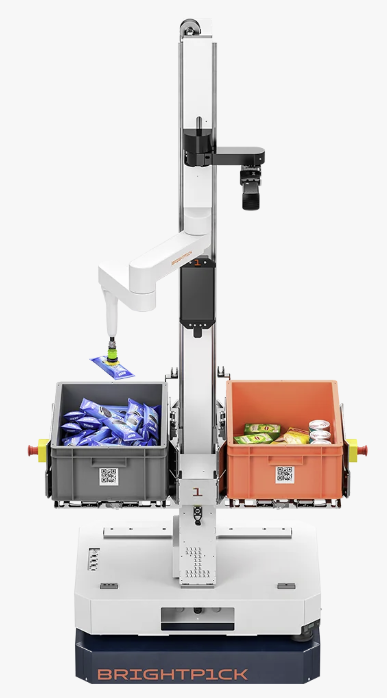
\includegraphics[width=90mm]{img/autopicker.png}
	\caption{Brightpick Autopicker }\label{OBRAZOK 1.2.1} 
\end{figure} 

Pre vývoj algoritmu plánovania trajektórie sa budeme zaoberať iba vybranou časťou tohoto komplexného riešenia a to konkrétne robotickým ramenom. Samotné robotické rameno sa skladá z 2 ramien a 2 rotačných kĺbov (obr. \ref{OBRAZOK 1.2.1}).  V porovnaní s klasickou kinematickou štruktúrou SCARA (obr. \ref{OBRAZOK 122}) nemá tretí rotačný kĺb, ktorý by zabezpečil rotáciu efektora - teda rotáciu samotného prenášaného objektu. Taktiež neobsahuje posuvný kĺb, ktorý by zabezpečil pohyb v smere osi $z$. Tento pohyb totiž zabezpečuje zdvižná plošina, na ktorej sú umiestnené krabice s tovarom. Pre potreby našej úlohy si teda kinematickú štruktúru môžeme zjednodušiť na 2 stupne voľnosti - 2 rotačné kĺby. Plánovanie trajektórie budeme riešiť len od bodu uchytenia objektu efektorom robota (počiatočný bod trajektórie) po dosiahnutie bodu uloženie objektu do krabice (koncový bod trajektórie). Toto obmedzenie nám umožní lepšie optimalizovať pohyb a zvážiť výhody a nevýhody kinematickej štruktúry.

Parametre robotického ramena sú uvedené v tabuľke  \ref{table 1.2}.  Parametre robota sa prejavujú v jeho pracovnom priestore (obr. \ref{OBRAZOK 123}), kde môžeme vidieť rozsah pohybu a dosiahnuteľných polôh nášho robotického ramena v 2D priestore.  Modrou farbou je označené prvé rameno, rozsah jeho pohybu je vyznačený rovnakou farbou. Druhé rameno robota je označené fialovou farbou, čo platí aj pre rozsah jeho pohybu. Všetky dosiahnuteľné polohy robotickým ramenom sú označené sivou farbou. Pracovný priestor robota aj s uchopeným prenášaným objektom je na obrázku označený červenou farbou. Tento priestor je určený rozmermi celého robota, konkrétne zdvižnou plošinou, ktorej sú umiestnené krabice s tovarom a objednávkou. Pri prenášaní objektu z jednej krabice do druhej nesmie objekt ani robotické rameno vyjsť z toho priestoru aby nedošlo ku kolízii, keďže mimo tohoto rozsahu nevieme zaručiť voľný priestor. 
\begin{table}[]
	\centering
	\begin{tabular}{|l|c|c|}
		\hline
		rameno   & \multicolumn{1}{l|}{dĺžka {[}mm{]}} & \multicolumn{1}{l|}{rozsah {[}rad{]}} \\ \hline
		link1 & 360                                 & 0 - $\pi$/2                              \\ \hline
		link2 & 260                                 & 0 - 2$\pi$                           \\ \hline
	\end{tabular}
	\caption{Parametre ramena}\label{table 1.2} 
\end{table}

\begin{figure}[]
	\centering
	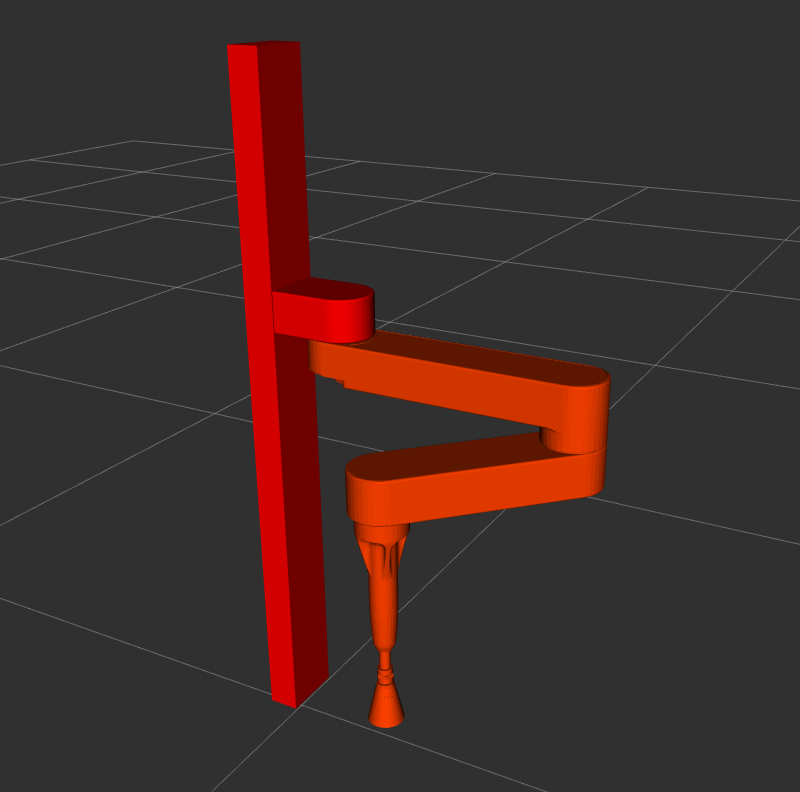
\includegraphics[width=80mm]{img/SCARA2.png}
	\caption{Model robota - Rviz}\label{OBRAZOK 122} 
\end{figure} 


\begin{figure}[]
	\centering
	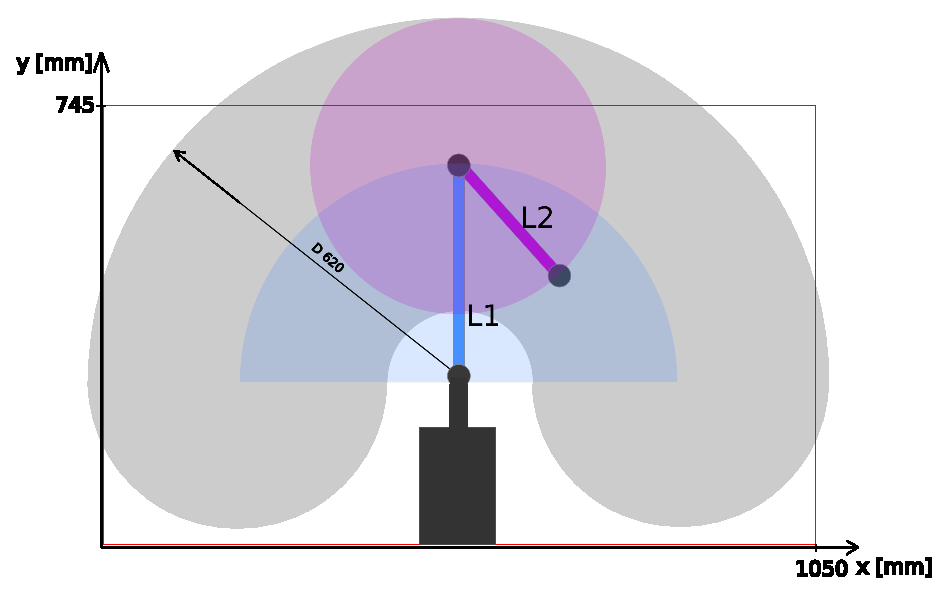
\includegraphics[width=140mm]{img/SCARA-workspace.eps}
	\caption{Pracovný priestor robotického ramena}\label{OBRAZOK 123} 
\end{figure} 

Aktuálnu kinematickú štruktúru robotického ramena je možné rozšíriť o ďalší rotačný kĺb, ktorý bude umiestnený v koncovej polohe druhého ramena. Táto úprava nám zvýši počet stupňov voľnosti robota, čo nám poskytne väčšie možnosti pohybu objektu v priestore. Tento nový kĺb umožní komplexnejšie manipulácie s objektmi a presnejšie umiestnenie, čo je kľúčové najmä v oblasti precíznej robotiky. Bližšie si predstavíme jednotlivé štruktúry v nasledujúcich podkapitolách \ref{kap:1.2.1} a \ref{kap:1.2.2}.


\subsubsection{2 stupne voľnosti}
\label{kap:1.2.1}

Prvou testovanou štruktúrou bude s 2 rotačnými kĺbmi , čo zodpovedá 2 stupňom voľnosti. V tejto kinematickej štruktúre sa budú otáčať 2 ramená robota a nástroj na uchytenie objektu , ktorý sa nachádza na konci kinematického reťazca bude fixný.
Pri tejto konfigurácii je kritické testovať schopnosť robota preniesť objekty rôznych tvarov a rozmerov zo štartovacej konfigurácie do cieľovej. Osobitnú pozornosť je potrebné venovať väčším podlhovastým objektom, kde môže nastať problém. Robot by mohol mať obmedzenú schopnosť otáčania objektov v rámci svojich dvoch rotácií ramien, čo by mohlo spôsobiť, že nedokáže dosiahnuť požadovanú konfiguráciu. Ďalším potenciálnym problémom môže byť kolízia so stĺpom, na ktorom je robotické rameno upevnené.

Testovanie na rôznych objektoch umožní identifikovať tieto obmedzenia a prípadne navrhnúť riešenia, ako ich prekonať. Zároveň bude možné získať dôležité informácie o výkonnosti a schopnostiach tohto typu kinematickej štruktúry v reálnych pracovných podmienkach.


\subsubsection{3 stupne voľnosti}
\label{kap:1.2.2}


Druhá testovaná kinematická štruktúra sa bude líšiť od prvej pridaním ďalšieho rotačného kĺbu, ktorý umožní otáčať nástrojom na uchytenie objektu. Táto úprava by mala výrazne zlepšiť schopnosť robota nájsť vhodnú trajektóriu pre presun objektu zo štartovacej do cieľovej pozície, pretože umožní flexibilnejšie a presnejšie nastavenie nástroja.

Dôležité je zaznamenať dáta, ktoré nám umožnia zhodnotiť, či pridaný rotačný kĺb prináša dostatočný prínos voči prvej konfigurácii. Tieto údaje nám pomôžu posúdiť, či investícia do efektívnejšieho robota s väčšími možnosťami je opodstatnená z hľadiska finančnej efektívnosti v porovnaní s lacnejším robotom, ktorý má obmedzené možnosti.

Kombinácia dosiahnuteľnosti cieľovej polohy pri rozličných rozmeroch objektov, časových dát a analýza efektivity bude kľúčová pri rozhodovaní, ktorá kinematická štruktúra je najvhodnejšia pre danú aplikáciu z hľadiska nákladov a výkonnosti. Získané informácie nám umožnia zvoliť optimálny dizajn robota, ktorý najlepšie vyhovie našim potrebám a požiadavkám.

